\documentclass[usenatbib]{mn2e}
\usepackage{mathpazo}

\usepackage{graphicx}
\usepackage{marginnote}
\usepackage{microtype}

\newcommand{\aspconf}{ASP Conf. Ser.}
% bold micron (for titles etc.
\newcommand{\bmicron}{\boldmath\ensuremath{\micron}}
% alternate micron command
\newcommand{\um}{\micron}

% referenceing commands
\newcommand{\sref}[1]{Sec.~\ref{#1}}

% commands and packages that shouldn't be needed in final version
\usepackage{xcolor, soul}
\newcommand{\todo}[1]{\textcolor{red}{TODO: #1}}
\newcommand{\note}[1]{\textcolor{red}{Note: #1}}
\newcommand{\ascl}[1]{\href{http://www.ascl.net/#1}{ascl:#1}}
\newcommand{\status}[1]{\textsf{#1}}

\title[SCUBA-2 850\um\ Legacy Release]%
{The JCMT Legacy Release: SCUBA-2 850\bmicron\ observations}

\author[S.~F.~Graves et~al.]
{Sarah~F.~Graves,$^{1,2}$
Graham~S.~Bell,$^{1,2}$
JAC
and
Others.\\
$^1$Joint Astronomy Centre, 660 N.\ A`oh\=ok\=u Place, Hilo, HI 96720, USA\\
$^2$East Asian Observatory, 660 N.\ A`oh\=ok\=u Place, Hilo, HI 96720, USA
}


\begin{document}

\date{in development}

\pagerange{\pageref{firstpage}--\pageref{lastpage}} \pubyear{2015}

\maketitle

\label{firstpage}

\begin{abstract}
  % Re write this properly once the rest of the paper is written.
  The JCMT Science archive allows access to raw and reduced data for
  all publicly available JCMT observations. To aid users of JCMT
  products, we have produced a standardised reduction of public JCMT
  SCUBA-2 850\,\um\ SCUBA-2 observations. These reductions provide
  uniformly reduced coadds of of all data that was public as of 2014 August
  1, and catalogues to identify the regions where emission was
  detected. The data have been gridded in the HEALPix HPX scheme.
\end{abstract}

\section{Introduction}
%\begin{itemize}
%\item Description of the JSA \citep{2015Economou}
%\item Very brief description of heterodyne and SCUBA-2 instruments, cite instrument papers. \citep{2013MNRAS.430.2513H} \citep{Buckle2009}
%\item Outline of the advanced data products. \citep{Bell2014}
%\item Historical perspective. \citep{Economou2011}
%\item ongoing plans -- dynamic archive, continually updated etc.
%\end{itemize}

% JCMT & SCUBA-2
The JCMT is a 15\,m submillimetre telescope located at an altitude of
4092\,m on Mauna Kea, where it has been operating since
1987. Its current instrument suite includes SCUBA-2, a 10,000
pixel continuum camera that observes simultaneously at 450\,\um\ and
850\,\um\ wavelengths\citep{Holland2013}.

% Whats in the Archive -- reductions using PI-chosen configurations
The JCMT Science Archive \citep{2015Economou}, hosted by the Canadian
Astronomy Data Centre (CADC) contains both raw, instrumental-format
data and pipeline-reduced FITS-format data. All science observations
from the observatory are reduced each night using the PI's chosen
configuration.  These reduced observations and co-adds are then
automatically made available in the archive (initially just to the PI
and coIs, but then publicly once the observations are no longer
proprietary). Although these project-specific configurations are vital
to ensure PI's can access the most scientifically useful reductions of
their data, it means that the reduced archival data is considerably
more heterogenous than some astronomical users may suspect, and
reduced observations of the same region of sky from different projects
cannot be naively co-added together. Despite this,
\citet{Bell2014} found that more than fifty percent of
papers using JCMT data made use of archive data.

To maximise the scientific return on the many years of archival data,
and to make it as easy as possible for non-submm-experts to use the
JCMT data, the Joint Astronomy Centre, then-operators of the JCMT,
decided to produce 'legacy' reductions of all public data from the
current instrumentation. These legacy reductions were envisioned as
providing a uniform, standardised reduction, co-addition and source
detection of all publicly available observations. The aim was to
produce uniformly reduced high quality co-added maps that required as
little checking as possible by hand, and would allow astronomers to
easily see at a glance what had been observed and detected on any
given region of the sky. This paper presents the first release in this
project: the 850\,\um\ SCUBA-2 continuum observations. Planned future
releases are the 450\,\um\ SCUBA-2 observations and the HARP spectral
observations in some of the most common molecular transitions.



\subsection{Observations included in this release}
% What data are included.

This release includes publicly-released 850\,\um\ science observations
observed between 2011 February 2 and 2013 August 1. Observations from
earlier than this were not included, as these were taken in
\emph{shared risk} mode while instrument commissioning was still being
conducted, and the data from that era are more problematic
\citep{SC19,Dempsey2010}.  Observations by the JCMT Cosmology Legacy
Survey \citep{Geach2013} are not included as they are still
proprietary until 2016 March 1. Observations by other SCUBA-2 JCMT Legacy
Surveys \citep[e.g.,][]{ChrysostomouJLS,GBS,SASSy,SONS,JPS}, as well as PI
projects from all queues, were included if they
fell in the given time range.
\note{Has any NGLS SCUBA-2 data been published? Need proper JPS and
  SASSy refs.}

Pointing observations, and observations from within the
appropriate time period that were judged to be of a low or
potentially-low quality, \emph{were} still reduced using this
standardised configuration\footnote{and are available for interested
  parties to download from the JSA}, but have not been included in the
co-added products (see \sref{sec:QA} for more detail on this).

10686 observations were reduced, of which 5165 are non pointing
observations included in these coadds, and 5521 were pointing
observations that were reduced but not coadded.

Of these 'science' observations, 49 observations were marked as 'bad'
and excluded from the coadds by our manual QA process.\footnote{A
  further 390 were marked as `Questionable'. This population were then
  examined further, and it was felt that these were all of high enough
  quality to include.}


\begin{table}
  \caption{Number and length of observations from various different
    categories of projects included in the coadded tiles in this
    release. \label{tab:obsnum}}
{\centering
\begin{tabular}{l r r r r}
  \hline
  Project Type &
  \multicolumn{1}{p{0.7cm}}{Num. obs.} &
  \multicolumn{1}{p{0.7cm}}{Obs. Time \newline(hrs)} &
  \multicolumn{1}{p{2.0cm}}{%
Percent of total obs.\ time\textsuperscript{*}}\\

  \hline

  All                      & 5115 & 2261 & 37\%   \\\\
  Calibrations             & 1103 &   81 & 52\%   \\\\
  Legacy Surveys (total)   & 1497 &  894 & 24\%   \\\\

  \hspace{0.5cm} CLS       & 0    &    0 &  0\%   \\
  \hspace{0.5cm} DDS/SONS  & 446  &  235 & 75\%   \\
  \hspace{0.5cm} GBS       & 342  &  236 & 57\%   \\
  \hspace{0.5cm} JPS       & 228  &  150 & 32\%   \\
  \hspace{0.5cm} NGS       & 169  &   68 & 38\%   \\\\

  Other projects  (total)  & 2459 & 1292 & 54\%   \\\\

  \hspace{0.5cm} Univ.~Hawaii   & 592 & 322 &  47\% \\
  \hspace{0.5cm} UK             & 956 & 524 &  58\% \\
  \hspace{0.5cm} Netherlands    & 161 &  45 & 100\%\\
  \hspace{0.5cm} Canada         & 497 & 359 &  75\%\\
  \hspace{0.5cm} International\textsuperscript{**}
                                 &35  &  19 &   9\%\\
  \hspace{0.5cm} Service        &   8 &   5 &  20\%\\
  \hspace{0.5cm} Directors      &  61 &  36 & 62\% \\
  \hspace{0.5cm} Staff Time     &  71 &  29 & 100\%\\
  \hline
\end{tabular}\\}
{\noindent\scriptsize \textsuperscript{*} The percentage of all
  SCUBA-2 time (from that type of project) which is included in the
  coadds. The calculation of total time for a given type of project
  does not include observations of moving targets, engineering
  observations, pointings or any non-science observations; it also
  does not filter out any observing time that is flagged as
  \status{JUNK} or \status{BAD} (these statuses are defined in \S\ref{sec:QA}). }

{\noindent\scriptsize \textsuperscript{**} Includes shared risk observations.}
\end{table}

\todo{ 1 more observation (JCMTCAL twoards CRL618) that won't reduce
  at the moment and should really be fixed, and coadd
  updated.. JobNumber 5804}

\subsection{Overview of Release}

\begin{figure*}
  \centering
  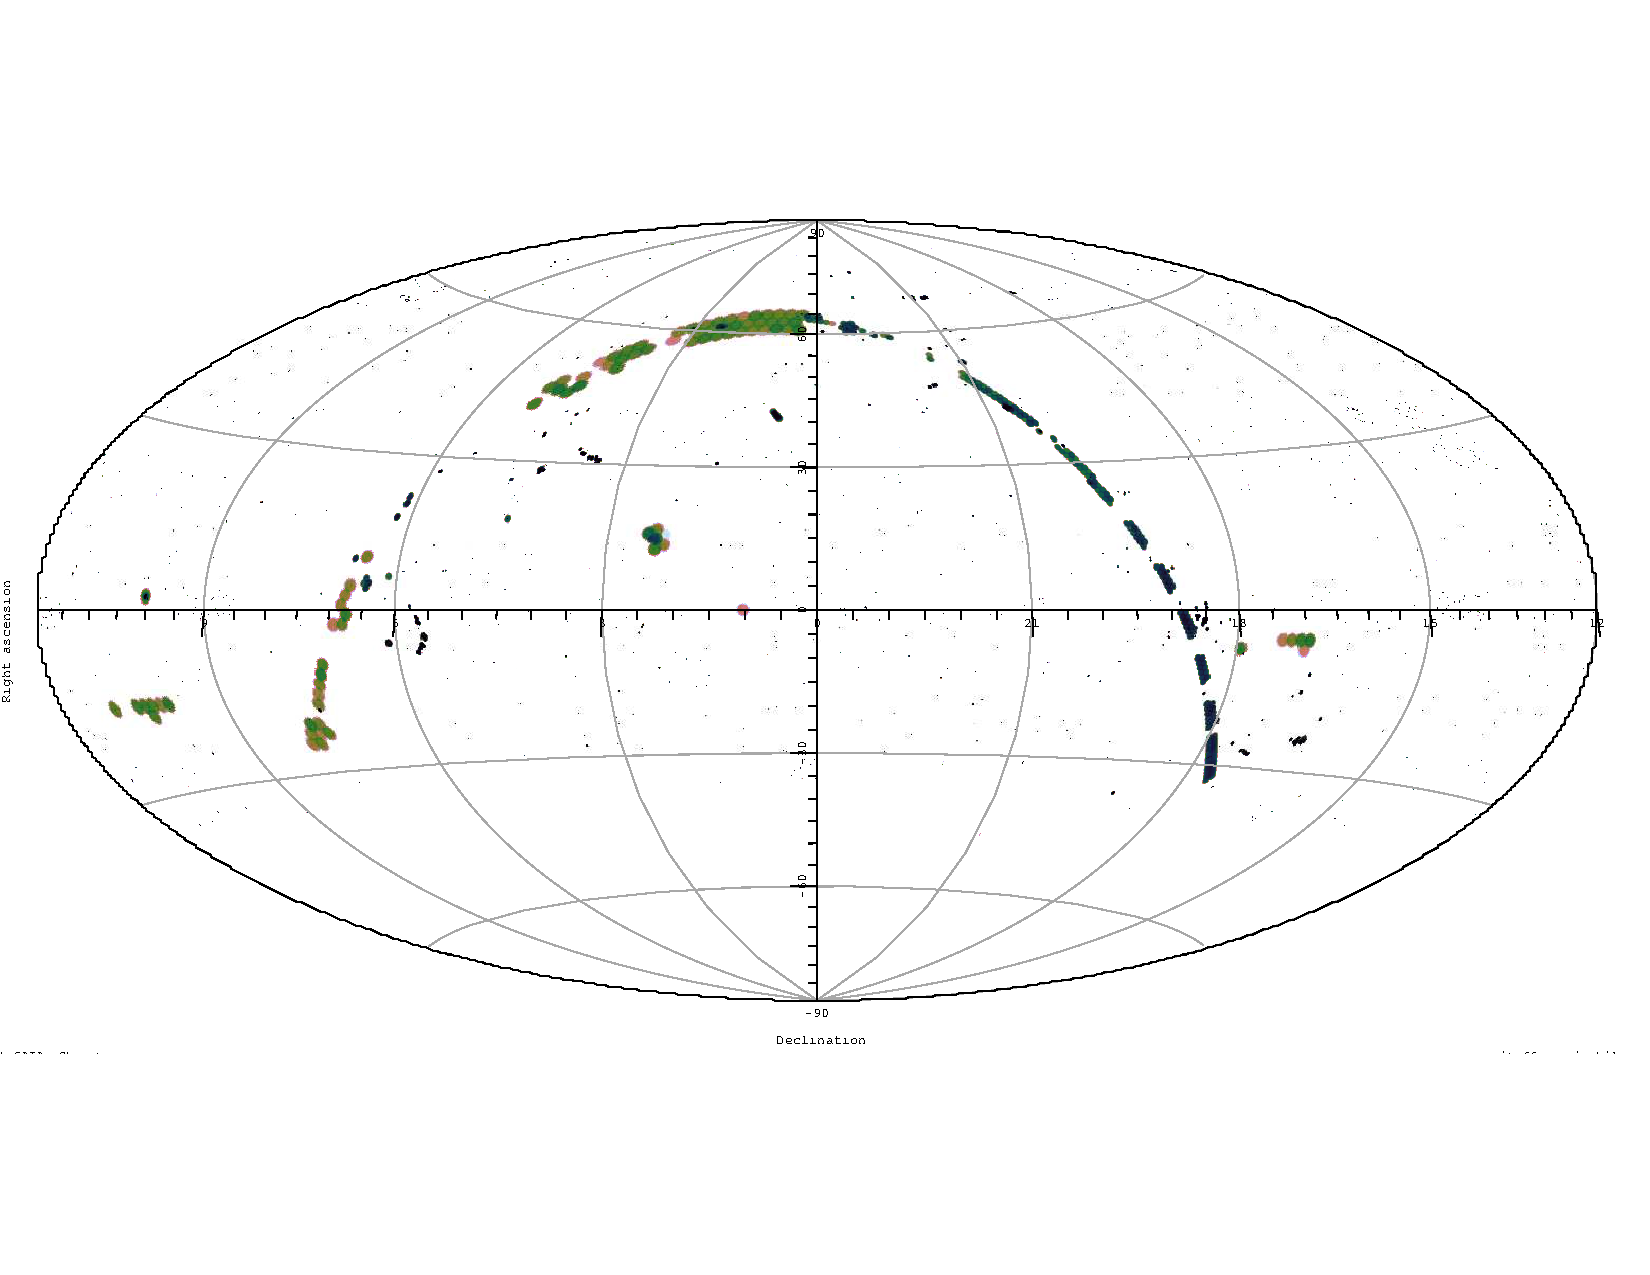
\includegraphics[width=0.9\linewidth]{legacy850-noise-aitoff}
  \caption{All sky noise map for this SCUBA-2 850um legacy
    release. The large circular regions are 1 and 2 degree pongs,
    predominately observed near the plane of the galaxy. Small points
    are daisy observations towards sources scattered across the
    sky.}
  \label{fig:noise-aitoff}
\end{figure*}

2849 tiles were produced,
% Number of observations included.

% Area covered.
% Number of islands of emission and peaks.

% Picture of areas covered in this release (noise map?)





\section{HEALPix grid }
Require a fixed tiling and grid to reduce our data onto, as we want to
be able to incorporate all data current and future into this
method. The chosen grid is that of the HEALPix method (Hierarchical
Equal Area isoLatitude pixelation), commonly used in cosmological
fields. This has the advantage that all pixels have the same area. The
trade off is that the pixels do not have the same size in RA and Dec.

\todo{GSB: Insert Brief Description of healpix, advantages and
  disadvantages and why it was chosen }

\todo{Create plots illustrating healpix}.

\todo{list parameters we have used}.

\footnote{To re-grid a HEALPix tile onto a standard RA-Dec projection,
  the Starlink \textsc{smurf} command \texttt{jsajoin} can be used
  \citep[][\ascl{1310.007}]{SUN258}.}

The Main HEALPix reference is \citep{Gorski2005}

Also see: ``Mapping on the HEALPix grid'' is \citep{Calabretta2007}



\section{SCUBA-2 data reduction}
Although all the JCMT observations were already being run through an
automated pipeline \citep{2011scuba2dr,2015oracdr}, these relied on the PI for a
project selecting the correct reduction `recipe'.

These recipes could produce very poor results when used on an
inappropriate observation -- for example, the standard SCUBA-2 recipe
used for calibrator observations is tuned to expect a bright, compact
source at the centre of the map, and if used by mistake on a blank
field this recipe could easily find \emph{fake emission} in the form
of large bloom-like structures. Avoiding this sort of erroneous result
was the paramount consideration when selecting the configuration
parameters.

Given the nature of SCUBA-2 data reduction algorithms, the main focus
in developing a configuration was placed on maximising the trust that
could be placed in detection of emission (based on simple SNR cuts),
at the expense of not attempting to recover large scale
structures.

% What version of the Starlink software was used to make this data
% release?
These observations were reduced using Starlink and
ORAC-DR software developed between versions 2014A and
2015A. Interested parties seeking to replicate these results can do
so with the 2015A release. \todo{CHECK THIS WORKS?}

\begin{itemize}
\item Brief description of how SCUBA-2 data reduction works.
\item mapmaker paper: \citep{Chapin2013}
\item Details of our chosen configuration and why we chose it. (detailed).
\item Examples of some reduced maps.
\end{itemize}

\subsection{Individual Observations}

\subsection{Co-adding of tiles}
All observations towards a given tile that passed QA were coadded,
using the \texttt{makemos} applications from Starlink's
\texttt{ccdpack} \citep[][\ascl{1403.021}]{SUN139}. This coadding was carried out as a variance-weighted
mean. No despiking was performed. The variance map for the coadded
tile is also produced.

\todo{Picture of a coadded tile? Both data and noise.}


\todo{Each observation is gridded into pre-defined tiles. Are they
  extinction corrected at that point? Unlike HARP processing
  \citep{2015ACSISDR}, observations can be reduced independently and
  then co-added. Extinction correction can be applied during coadding
  phase? How well are edge-effects handled by variance weighting?}


\section{QA}
\label{sec:QA}
\subsubsection{Standard JCMT QA States}
All observations taken by the JCMT are classified as \status{GOOD} (the
default), \status{BAD}, \status{QUESTIONABLE}, \status{JUNK} or \status{REJECTED}. We included
\status{GOOD}, \status{QUESTIONABLE} and \status{REJECTED} data in our co-adds. The \status{REJECTED}
state is used by the JLS teams to indicate that a particular
observation did not meet their particular QA criterion but the data
are otherwise usable. The \status{QUESTIONABLE}
state was originally designed to be a transient state that would be
resolved into either \status{BAD} or \status{GOOD} after analysis, but in practical
terms there was not a work flow to ensure this, so some observations
have this flag in the archive.

Usually (in the standard nightly reduction pipelines) \status{QUESTIONABLE}
data is treated as if it is \status{BAD} for the purposes of co-adds. However,
due to our second QA stage for this release, we chose to include it as
long as it passed our special legacy QA.

\subsection{Legacy Release QA}
%Description of process. Examples of observations we threw out.

Every reduced file included in this has been marked as \status{GOOD} by a
member of the JAC team. This quick 'by-eye' assessment was simply done
on a image of the reduced map. This QA process was designed to avoid:
a) `blooms' or `blobs' of fake emission that can sometimes be produced
at the edges of the map by the mapmaker.  b) identify the most
problematic observations that had missed being flagged under the
telescope standard QA process.

This sort of process is of course subjective, and some of the
observations that we excluded might turn out fine on further
examination. However, as with all of this process, the focus for this
release has been to pursue ensure a high quality, even at the expense
of completeness. All of the HEALPix-gridded legacy-reduced
observations are available to the community in the JSA, regardless of
our QA analysis of them.


\section{Calibration}
\begin{itemize}
\item Calibration paper \citep{Dempsey2013}
\item show images the standard calibrators.
\item comparison with 'standard' calibrator reductions
\item effect of pixel size on fluxes. Per, Jess \& Daniel may have
  something. Doug J. and GBS did an analysis on this as well.
\item effect of pointing errors on fluxes.
\item Our uncertainty in the final flux.
\end{itemize}


We calibrated our data into units of mJy per arc-second squared, using
the standard FCF values from \citet{Dempsey2013}.  As the
effective beam size is increased during the co-add procedure (due to
errors in the pointing between different maps), and the choice of
pixel size will also affect the effective beam size of the final map,
we have chosen not to try and calibrate into units of the beam.


\section{Bowling}
Examples of the bowling in our maps.

\section{Noise}
\begin{itemize}
\item Analysis of the noise maps, how believable they are.
\item High noise towards bright sources.
\end{itemize}



\section{Catalogues}
\begin{itemize}
\item CUPID \citep{cupid} Fellwalker! \citep{Berry2015}
\item Island and peak paradigm overview.
\item Details of our chosen parameters
\item Cross referencing between neighbouring tiles.
\end{itemize}


\section{Robustness of products}
% NB improve this section title.

\subsection{Source Recovery: Comparison including fake sources?}
cf Steve Mairs GBS paper (in prep)
\note{ probably merge this and previous subsection}

\subsection{Size Scales}

\section{Comparison with legacy surveys}

\todo{A SCUBA-2 image from each survey alongside a Legacy Release
  version. Which wavelengths? SASSy only has one published field
  \citep{MacKenzie2011}. JPS and NGLS may not have any yet. GBS has a
  few recent papers with \citet{Rumble2015} published for Serpens.}

\section{Accessing the Legacy Release}
A brief summary of how to access the data, catalogues, any cool tools
we've found/developed before the release etc.

\section{Conclusions}

\section*{Acknowledgments}

The James Clerk Maxwell Telescope has historically been operated by
the Joint Astronomy Centre on behalf of the Science and Technology
Facilities Council of the United Kingdom, the National Research
Council of Canada and the Netherlands Organisation for Scientific
Research. This work was funded by the Science and Technology Facilities
Council.

\bibliography{legacy-850um-paper}
\bibliographystyle{mn2e}

\appendix
\onecolumn

%% Probably more detailed than needed in a paper
\section{Mapmaker configuration}
The mapmaker configuration used for this release (known as a
\texttt{dimmconfig}) is shown here. Like most SCUBA-2 mapmaker
configuration files, it first sources the \emph{base}
\texttt{dimmconfig} file that sets up the basic values for a range of
options and then tweaks a subset of additional parameters or its
purposes. This file is shipped in the 2015A Starlink release. The
value of every configuration parameter used is written into the
history component of the file.

\begin{verbatim}
^$STARLINK_DIR/share/smurf/dimmconfig.lis

#  Less aggressive cleaning to cope with bright sources
noisecliphigh=10.0
dcthresh = 100

#  Don't want extended structure, so avoid problems with COM model by using
#  individual common-mode models for each subarray.
com.perarray = 1

#  Aggressive filtering.
flt.filt_edge_largescale=200

#  Allow bolometer noise to vary with time, and using a box filter to
#  determine mean noise in each box, in order to presevre as many samples
#  as possible.
noi.box_size=-15
noi.box_type=1

#  Use a maximum of 20 iterations
numiter=-25
maptol_mean=1
maptol=0.01

# new recommendations and using an ast model
ast.zero_snr = 5
ast.zero_snrlo = 3

ast.skip=5
flt.zero_snr=5
flt.zero_snrlo=3
\end{verbatim}


\label{lastpage}
\bsp


\end{document}
